\chapter{Experimental Setup}

\MyQuote{To confine our attention to terrestrial matters would be to limit the
human spirit.}{Stephen Hawking}

In the previous chapter, the key features of QCD - today's theory of strong
interaction, were introduced. The predictions of QCD are tested at particle
accelerators persistently and there is the whole army of theoretical physicists
waiting for discovery of new phenomenon in which explanation QCD will fail.
Unfortunately for them, there is no such measurement which would not be in
agreement with QCD predictions up to date. 

In this chapter, the QCD will be raised from the theoretical description of the
previous chapter, to the practical implementation on Large Hadron Collider
(LHC). The LHC will be described with emphasize on the ATALS detector, which
data was used in this thesis. The all important concept of particle physics of
hadron colliders - jet - will be introduced in this chapter.

\section{The Large Hadron Collider and ATLAS Detector}

\subsection{The Large Hadron Collider}

The Large Hadron Collider (LHC) \cite{LHC, LHCPastPresentFuture} is a charged
particle accelerator located on the border of France and Switzerland, near
Geneva. Built using the areas of the Large Electron-Positron collider, the main
accelerator ring, of a 27 km circumference, is located around 100 m below the
surface. There are four main experiments located around the ring: A Large Ion
Collider Experiment (ALICE), A Toroidal LHC ApparatuS (ATLAS), Compact Muon
Solenoid (CMS) and Large Hadron Collider beauty (LHCb). The complete accelerator
and detector system is shown at Figure (?figure?).

LHC started to operate on November 23, 2009 and soon thereafter (March 30, 2010)
the proton-proton collisions achieved the center-of-mass energy $\sqrt{s} = 7
\TeV$, which is halve of the design energy of the machine. On April 5, 2012, the
machine started its successful $\sqrt{s} = 8 \TeV$ run.

Next to the proton-proton collisions first heavy-ion Pb-Pb collisions took place
in 2010 at a center of mass energy per pair of colliding nucleons $\sqrt{s} =
2.76 \TeV$. Proton-Pb collisions at $\sqrt{s} = 5.02 \TeV$ occurring on LHC
during 3 weeks of 2013, successfully demonstrated LHC capability to provide
asymmetric collisions.  

??? The accelerator complex is currently being upgraded, and so are the LHC
experiments. The machine will be back in 2015 with proton-proton collisions at
$\sqrt{s} \sim 13 \TeV$. Switching the beam crossing time from the current $50
\, \mbox{ns}$ to a $25 \, \mbox{ns}$ is still under consideration.

\subsection{The ATLAS Detector}

The ATLAS detector \cite{ATLAS} is a general-purpose detector surrounding one of
the interaction points of the LHC and with $\sim 100$ million of individual
electronic channels it is the most complicated instrument ever created having
one simple task: Record charged particle collisions up to the center-of-mass
energy per pair of colliding nucleons $\rts = 14 \TeV$. A detector overview is
shown in Figure~\ref{fig:ATLASfull}, where the main sub-detector systems can be
seen: the inner detector, used to reconstruct charged-particle tracks, the
electromagnetic calorimeters, the hadronic calorimeters, and the muon
spectrometer. 

\begin{figure}[t]
  \centering
  \begin{subfigure}[b]{0.8\textwidth}
    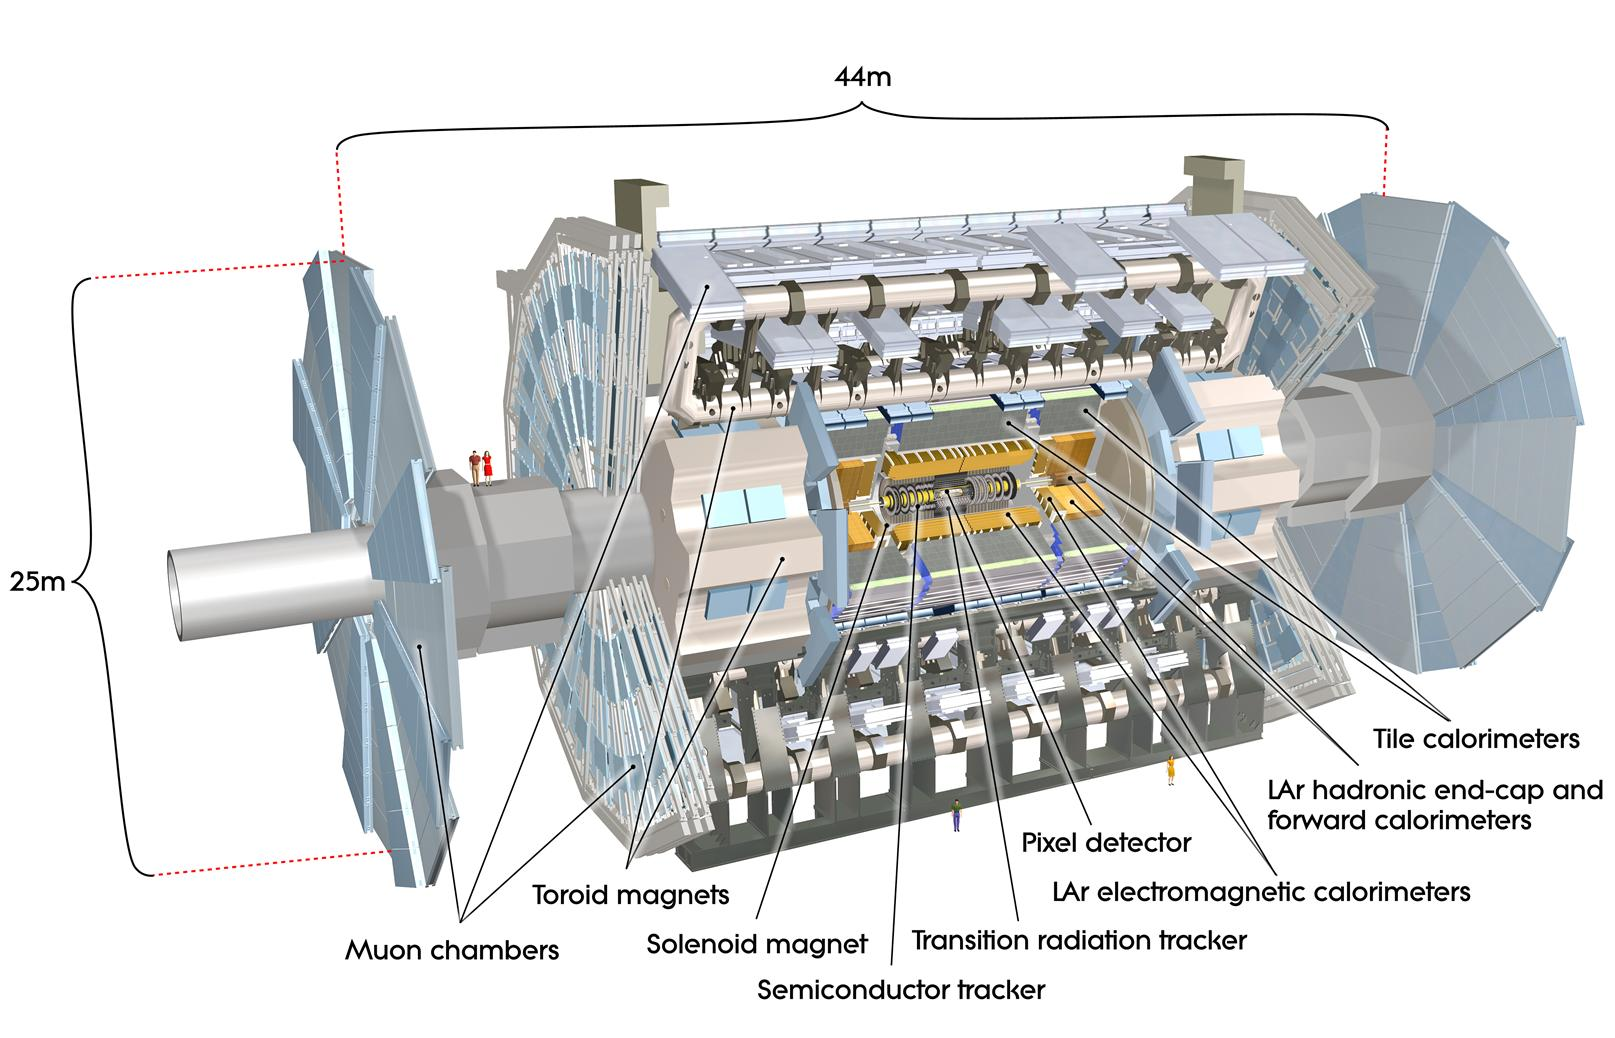
\includegraphics[width=\textwidth]{Chapter2/ATLAS.png}
    \caption{ATLAS detector}
    \label{fig:ATLASfull}
  \end{subfigure}
  ~
  \begin{subfigure}[b]{0.8\textwidth}
    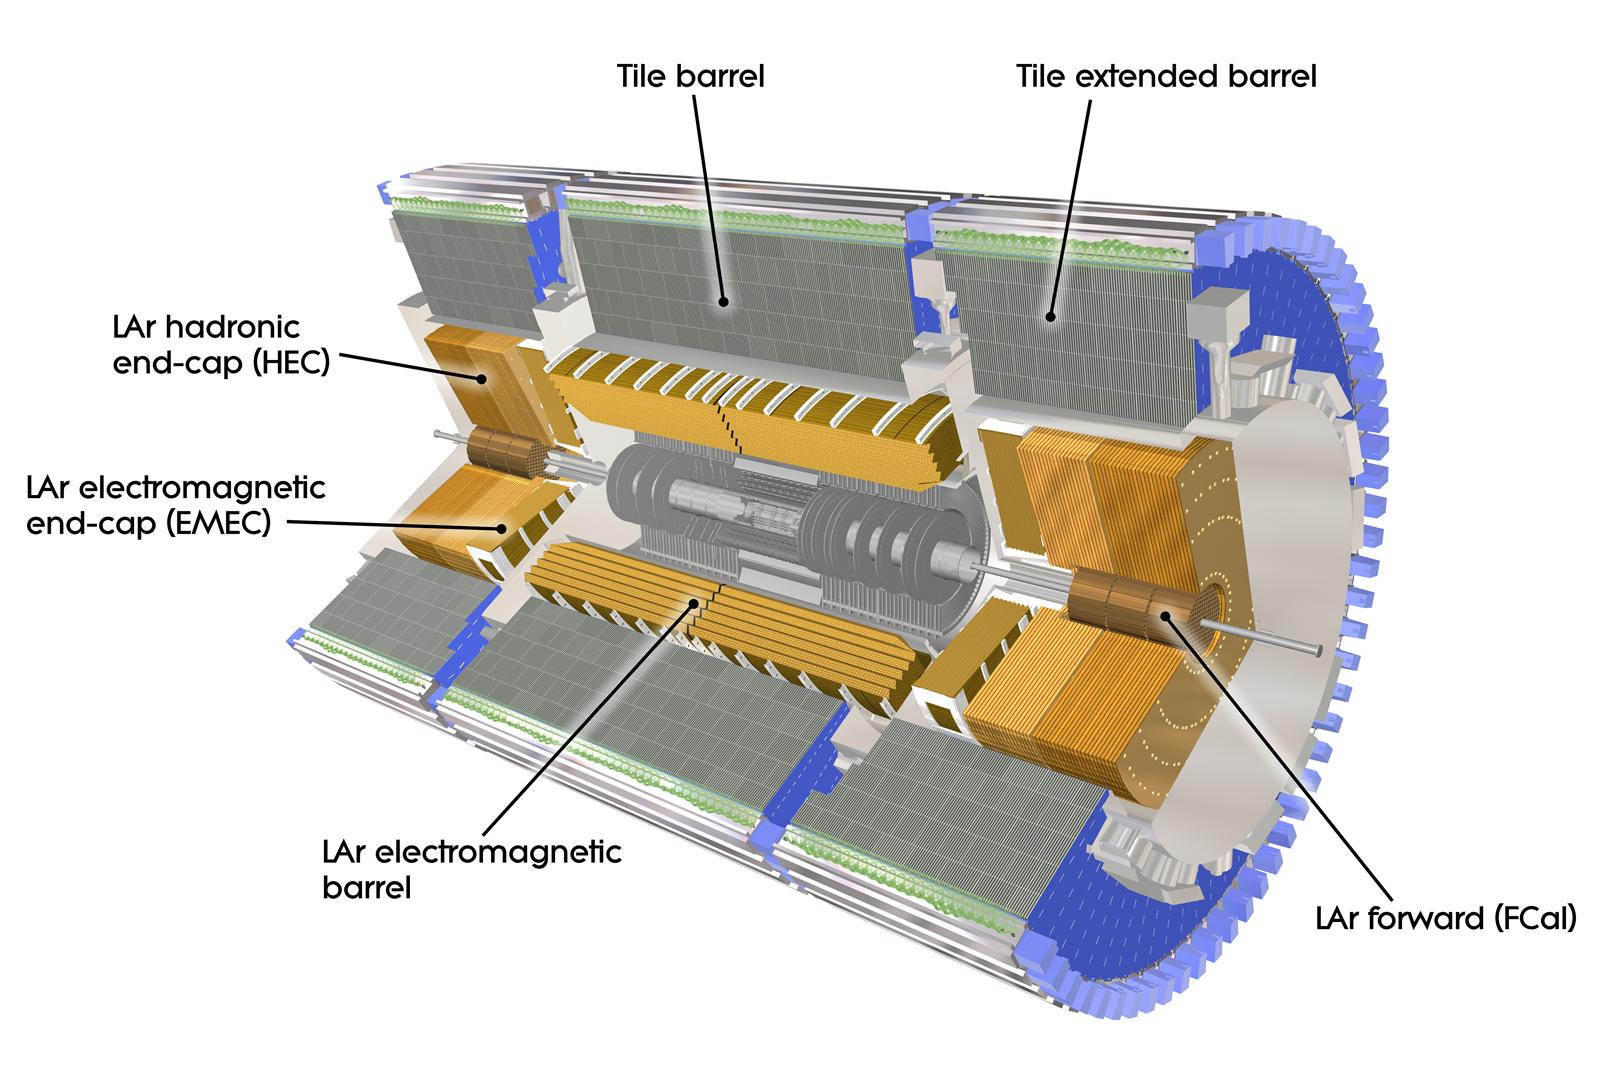
\includegraphics[width=\textwidth]{Chapter2/ATLASinner.jpeg}
    \caption{Inner detector and calorimeter systems}
    \label{fig:ATLASinner}
  \end{subfigure}
  \caption{(a) an overview of the ATLAS detector 
           (b) detail on the inner detector and the calorimeters - the dominant
           sub-detector systems used in this paper. Figures from
           \cite{CERNbook}.}
  \label{fig:ATLAS}
\end{figure}

ATLAS uses a right-handed coordinate system with its origin at the interaction
point in the center of the detector and the $z$ axis along the beam pipe. The
$x$ axis points from the interaction point to the center of the LHC ring, and
the $y$ axis points upward. Cylindrical coordinates $(r, \phi)$ are used in the
transverse plane, $\phi$ being the azimuthal angle around the beam pipe. Instead
of polar angle $\theta$ pseudorapidity $\eta$ is used throughout this paper. For
event selection the rapidity $y$ plays an important role. In following
definitions of pseudorapidity $\eta$ and rapidity $y$, $E$ stands for the total
energy and $p$ for size of total momentum: 
\begin{eqnarray}
  \eta &= & - \frac{1}{2} \ln \left( \frac{p+p_z}{p-p_z} \right) = - \ln \left[
  \tan \left( \frac{\theta}{2} \right) \right], \\ y &= &- \frac{1}{2} \ln
  \left( \frac{E+p_z}{E-p_z} \right).	
\end{eqnarray}
The transverse momentum $\pt$ presents the component of momentum perpendicular
to the beam line.  

The main detector system relevant to this thesis is the ATLAS calorimeter,
which is emphasized in Figure~\ref{fig:ATLASinner}. The calorimeter is divided
into sub-detectors, providing overall coverage up to $|\eta| < 4.9$. The
electromagnetic calorimeter, covering region $|\eta| < 3.2$, is a
high-granularity sampling detector in which the active medium is liquid argon
(LAr) interspaced with layers of lead absorber. The hadronic calorimeters are
divided into three sections: a tile scintillator/steel calorimeter is used in
both the barrel ($|\eta| < 1.0$) and extended barrel cylinders ($0.8 < |\eta| <
1.7$) while the hadronic endcap ($1.5 < |\eta| < 3.2$) consists of LAr/copper
calorimeter modules. The forward calorimeter measures both electromagnetic and
hadronic energy in the range $3.2 < |\eta| < 4.9$ using LAr/copper and
LAr/tungsten modules. 

%Energy resolution of ATLAS calorimeter \cite{JetEnergyResolution} is $\sim
%15\,\%$ for jets with energies in the range $20 \GeV < E < 50 \GeV$ and
%decreases to $\sim 5\,\%$ for jets with energies $E > 1 \TeV$. Jet energy
%resolution is generally better in lower pseudorapidity regions. 

\section{Hadron Collision at LHC}

Describe what happens when hadrons collide - this will lead to definitions of
jets

A jet can be naively seen as a group of collimated particles generated by the
hadronisation of a parton in the scattering process.

\section{Jet Algorithms}

Jet algorithm is a generic "recipe" which takes a set of particles (with defined
four-momenta) and returns jets created from them. That recipe usually involves a
set of parameters which together with the recipe fully specify the jet
definition. 

Principals of two jet algorithms are described here - fixed cone algorithm and
$k_t$ algorithm. First of these algorithms is more illustrative, the second one
is used in ATLAS. Detailed description as well as other jet algorithms can be
found in \cite{ATLASmain}. After definitions of jet algorithms it is shortly
described, how the objects (not necessary particles) with defined four-momenta
are constructed from the signal observed on the ATLAS detector. 

\subsection{Fixed cone algorithm}

The first step of this algorithm is to order all input objects (reconstructed
detector objects with four-momentum representation) in decreasing order in
transverse momentum $\pt$. If the object with the highest $\pt$ is above the
seed threshold, all objects within a cone in pseudorapidity $\eta$ and azimuth
$\phi$ with $\Delta R = \sqrt{\Delta \eta^2 + \Delta \phi^2} < R_{cone}$, where
$R_{cone}$ is the fixed cone radius, are combined together. A new direction is
calculated from the four-momenta inside the initial cone and a new cone is
centered around it. Objects are then recollected in this new cone and again the
direction is updated. This process continues until the direction of the cone
does not change anymore after recombination, at which point the cone is
considered stable and is called a jet. At this point, the next seed is taken
from the input list and a new cone jet is formed with the same iterative
procedure. This continues until no more seeds are available. 

The jets found this way can share some constituents. This algorithm is not
infrared safe. It means, that the presence of additional soft particles between
two particles belonging to the same jet can affect the recombination of these
two particles into a jet. In the same sense, the absence of additional soft
particles between these two can disturb the correct reconstruction of the jet.
This is ilustrated in Figure~\ref{fig:IRsafety}.

\begin{figure}[t]
  \centering
  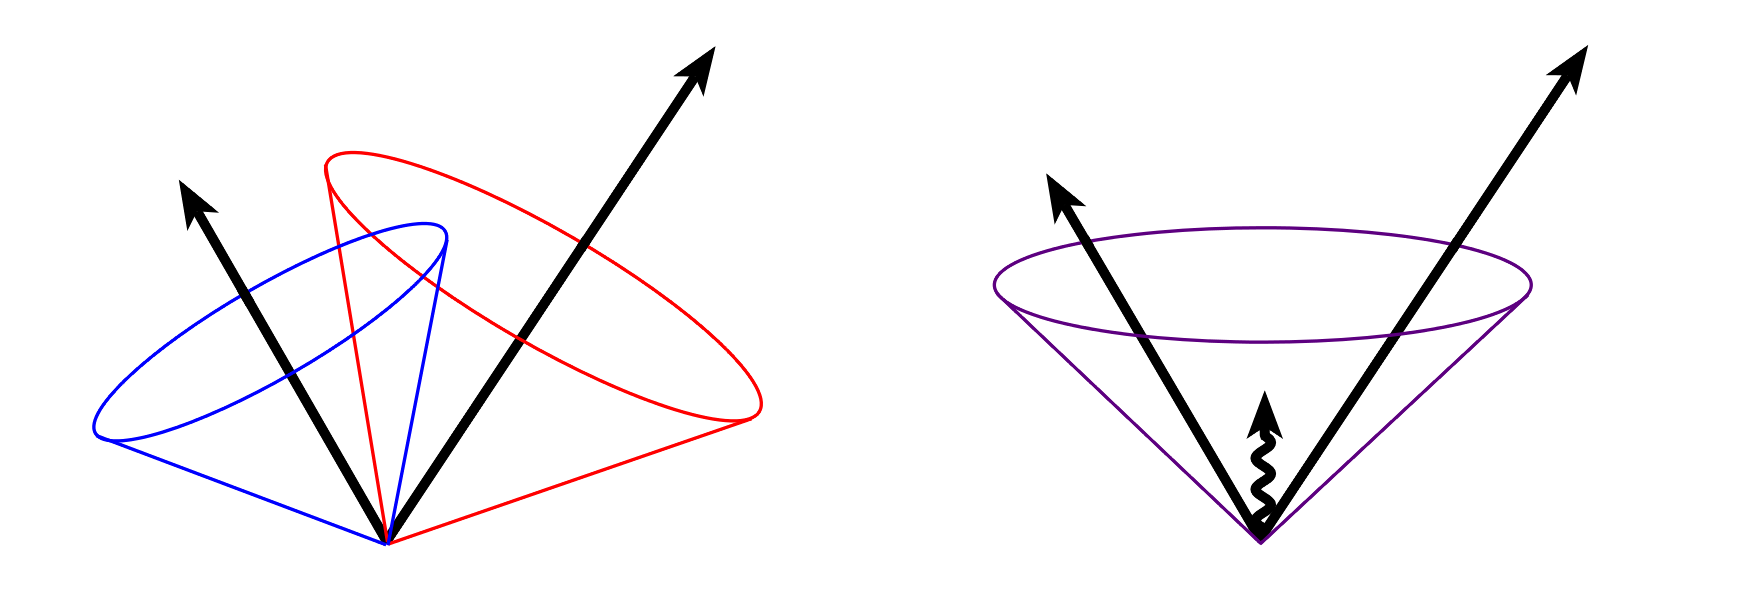
\includegraphics[width=\textwidth]{Chapter2/IRsafety}
  \caption{Fixed cone algorithm is not infrared safe - soft particle between two
  hard particles can determine, if hard particles end in different jets or will
  be part of the same one.} \label{fig:IRsafety}
\end{figure}

Parameters used by fixed cone algorithm are a seed threshold of $\pt > 1 \GeV$,
and a narrow ($R_{cone} = 0.4$) or a wide cone jet ($R_{cone} = 0.7$) option.

\subsection{$k_t$ algorithms}

In this class of algorithms all pairs $(i,j)$ of input objects are analyzed with
respect to their relative transverse momentum squared, defined by 

\begin{equation}
	d_{ij} = \min{\left( p_{T,i}^{2p} , p_{T,j}^{2p} \right)} \frac{\Delta R_{ij}^2}{R^2}
\end{equation}
and the squared $\pt$ of object $i$ relative to the beam axis

\begin{equation}
	d_i = p_{T,i}^{2p}.
\end{equation}
Here $\Delta R_{ij}^2 = (y_i - y_j)^2 + (\phi_i - \phi_j)^2$ and $p_{T,i}$,
$y_i$ and $\phi_i$ are respectively the transverse momentum, rapidity and
azimuth of particle $i$. In addition to the radius parameter $R$, parameter $p$
was added to split $k_t$~algorithms into three categories.  
\begin{itemize}
	\setlength{\itemsep}{0pt}
	\setlength{\parskip}{0pt}
	\setlength{\parsep}{0pt}
	\item $p = 1$ $k_t$ algorithm,
	\item $p = 0$ Cambridge/Aachen algorithm,
	\item $p = -1$ anti-$k_t$ jet-clustering algorithm.
\end{itemize}
The differences between these algorithms are detailed described in~\cite{ANTIKT}.  

These algorithms first find the minimum $d_{min}$ of all $d_{ij}$ and $d_i$. If
$d_{min}$ is in $d_{ij}$'s, the corresponding objects $i$ and $j$ are combined
into a new object $k$ using four-momentum recombination. Both objects $i$ and
$j$ are removed from the list, and the new object $k$ is added to it.

If $d_{min}$ is in $d_i$'s, the object $i$ is considered to be a jet by itself
and removed from the list.

This means that all original input objects end up to be either part of a jet or
to be jets by themselves. Contrary to the cone algorithm described earlier, no
objects are shared between jets and the procedure is infrared safe.

ATLAS uses anti-$k_t$ algorithm with $R=0.4$ for narrow and $R=0.6$ for wide
jets.

\subsection{Calorimeter jets}

The most important detectors for jet reconstruction are the ATLAS calorimeters.
The ATLAS calorimeter system has about 200,000 individual cells of various sizes
and with different readout technologies and cell geometries. For jet finding it
is necessary to first combine these cell signals into larger signal object with
physically meaningful four-momenta. The two concepts available are calorimeter
signal towers and topological cell clusters.

In the case of calorimeter signal towers, the cells are projected onto a fixed
grid in pseudorapidity $\eta$ and azimuth $\phi$. The tower bin size is $\Delta
\eta \times \Delta \phi = 0.1 \times 0.1$ in the whole acceptance region of the
calorimeters, i.e. in $|\eta| < 5$ and $- \pi < \phi < \pi$ with $100 \times 64
= 6,400$ towers in total.

The alternative representation of the calorimenter signals for jet
reconstruction are topological cell clusters, which are basically an attempt to
reconstruct three-dimensional "energy blobs" representing the showers developing
for each particle entering the calorimeter. The clustering starts with seed
cells with a signal-to-noise ratio, or signal significance $\Gamma = E_{cell} /
\sigma_{noise,cell}$, above a certain threshold $S$, i.e. $|\Gamma| > S = 4$.
All directly neighbouring cells of these seed cells, in all three dimensions,
are collected into the cluster. Neighbours of neighbours are considered for
those added cells which have $\Gamma$ above a certain secondary threshold $N$
($|\Gamma| > N = 2$). Finally, a ring of guard cells with signal significances
above a basic threshold $|\Gamma| > P = 0$ is added to the cluster. After the
initial clusters are formed, they are analyzed for local signal maximums by a
splitting algorithm, and split between those maximums.



\section{Jet Reconstruction}

How the jets are reconstructed including description of their calibration.
